\documentclass[12pt,a5]{bxjsarticle}

\usepackage{xltxtra}
\setmainfont{IPAPMincho}
\setsansfont{IPAPGothic}
\setmonofont{IPAGothic}
\XeTeXlinebreaklocale "ja"

\usepackage{hyperref}
\usepackage{listings}
\usepackage{verbatim}

\newcommand{\e}{\mathrm{e}}

\title{物理学情報処理論2 problem3}
\date{}

\begin{document}
\maketitle

$ | 1 + z + \frac{z^2}{2} | \le 1 $, $ | 1 + z + \frac{z^2}{2} + \frac{z^3}{6} + \frac{z^4}{24} | \le 1 $ の領域の境界の形

problem3\_1.cppでは、$ [-2, 0] $ の範囲でdxごとにyの符号の変化する点を探した。
problem3\_2.cppでは、問2と共にサンプルの通り$ (-0.5, 0) $を中心とする極座標で初めて符号の変化する点を探した。

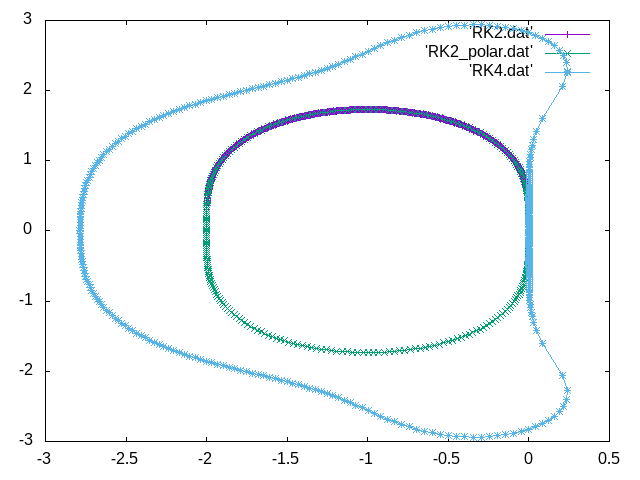
\includegraphics[width=\linewidth]{orbit.png}

以下のスクリプトを用いて、orbit.datから図を生成した。
\lstinputlisting[caption=plot.sh,language=bash]{plot.sh}

\end{document}
